\documentclass[tikz,border=4pt]{standalone}
\usepackage{tikz}
\usepackage{amsmath}
\usetikzlibrary{arrows.meta,calc,positioning,shapes.geometric,backgrounds,fit,patterns}

\begin{document}
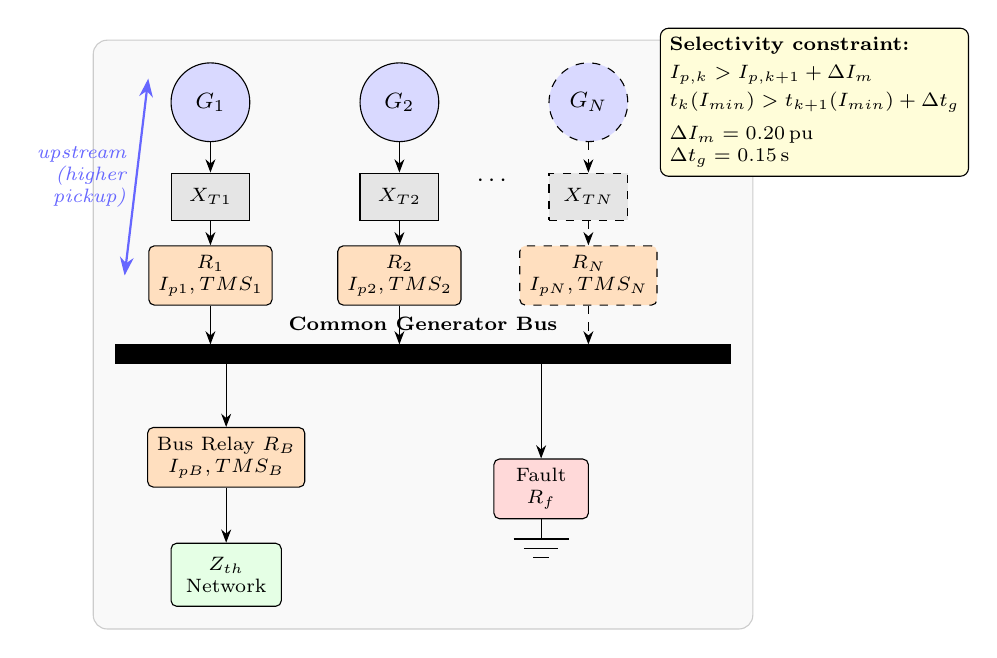
\begin{tikzpicture}[
  font=\small,
  >=Stealth,
  gen/.style ={draw,circle,minimum size=1.0cm,fill=blue!15,align=center,
               font=\footnotesize},
  xfmr/.style={draw,rectangle,minimum width=1.0cm,minimum height=0.6cm,
               fill=gray!20,align=center,font=\scriptsize},
  relay/.style={draw,rectangle,minimum width=1.1cm,minimum height=0.6cm,
                fill=orange!25,align=center,font=\scriptsize,rounded corners=2pt},
  bus/.style ={draw,rectangle,fill=black,minimum width=7.8cm,minimum height=0.15cm},
  load/.style={draw,rectangle,minimum width=1.4cm,minimum height=0.7cm,
               fill=green!15,align=center,font=\scriptsize,rounded corners=2pt},
]

%% =====================================================
%%  Main bus (horizontal)
%% =====================================================
\node[bus] (bus) at (3.5,0) {};
\node[above=0.05cm of bus,font=\scriptsize\bfseries] {Common Generator Bus};

%% =====================================================
%%  Generator 1 (left side)
%% =====================================================
\node[gen]   (g1)   at (0.8, 3.2) {$G_1$};
\node[xfmr]  (t1)   at (0.8, 2.0) {$X_{T1}$};
\node[relay]  (r1)   at (0.8, 1.0) {$R_1$\\$I_{p1},TMS_1$};

\draw[->] (g1.south)  -- (t1.north);
\draw[->] (t1.south)  -- (r1.north);
\draw[->] (r1.south)  -- (bus.north-|r1.south);

%% =====================================================
%%  Generator 2 (centre-left)
%% =====================================================
\node[gen]   (g2)   at (3.2, 3.2) {$G_2$};
\node[xfmr]  (t2)   at (3.2, 2.0) {$X_{T2}$};
\node[relay]  (r2)   at (3.2, 1.0) {$R_2$\\$I_{p2},TMS_2$};

\draw[->] (g2.south)  -- (t2.north);
\draw[->] (t2.south)  -- (r2.north);
\draw[->] (r2.south)  -- (bus.north-|r2.south);

%% =====================================================
%%  Generator N (right, dashed for general N)
%% =====================================================
\node[gen,dashed]   (gN)   at (5.6, 3.2) {$G_N$};
\node[xfmr,dashed]  (tN)   at (5.6, 2.0) {$X_{TN}$};
\node[relay,dashed]  (rN)   at (5.6, 1.0) {$R_N$\\$I_{pN},TMS_N$};

\draw[->,dashed] (gN.south)  -- (tN.north);
\draw[->,dashed] (tN.south)  -- (rN.north);
\draw[->,dashed] (rN.south)  -- (bus.north-|rN.south);

\node at (4.4,2.2) {$\cdots$};

%% =====================================================
%%  Downstream bus relay + Thevenin network
%% =====================================================
\node[relay,below=0.8cm of bus,xshift=-2.5cm] (rbus)
      {Bus Relay $R_B$\\$I_{pB},TMS_B$};

\coordinate (busout) at ($(bus.south)+(-2.5cm,0)$);
\draw[->] (busout) -- (rbus.north);

\node[draw,fill=green!10,minimum width=1.4cm,minimum height=0.8cm,
      align=center,font=\scriptsize,rounded corners=2pt,
      below=0.7cm of rbus] (zth) {$Z_{th}$\\Network};
\draw[->] (rbus.south) -- (zth.north);

%% =====================================================
%%  Fault branch
%% =====================================================
\coordinate (faultpt) at ($(bus.south)+(1.5cm,0)$);
\node[draw,fill=red!15,minimum width=1.2cm,minimum height=0.6cm,
      align=center,font=\scriptsize,rounded corners=2pt,
      below=1.2cm of faultpt] (fault) {Fault\\$R_f$};
\draw[->] (faultpt) -- (fault.north);

% Ground
\coordinate (gnd) at ($(fault.south)+(0,-0.25)$);
\draw (fault.south) -- (gnd);
\draw ($(gnd)+(-0.35,0)$) -- ($(gnd)+(0.35,0)$);
\draw ($(gnd)+(0,-0.12)+(-0.22,0)$) -- ($(gnd)+(0,-0.12)+(0.22,0)$);
\draw ($(gnd)+(0,-0.24)+(-0.10,0)$) -- ($(gnd)+(0,-0.24)+(0.10,0)$);

%% =====================================================
%%  Coordination constraint annotation
%% =====================================================
\node[draw,fill=yellow!15,rounded corners=3pt,
      right=0.4cm of gN,align=left,font=\scriptsize,
      minimum width=3.4cm] (coord)
      {\textbf{Selectivity constraint:}\\[2pt]
       $I_{p,k} > I_{p,k+1} + \Delta I_m$\\[2pt]
       $t_{k}(I_{min}) > t_{k+1}(I_{min}) + \Delta t_g$\\[4pt]
       $\Delta I_m = 0.20\,\text{pu}$\\
       $\Delta t_g = 0.15\,\text{s}$};

%% =====================================================
%%  Upstream/downstream arrow
%% =====================================================
\draw[<->,thick,blue!60] (r1.west)+(-0.3,0) -- node[left,font=\scriptsize\itshape,
     align=right]{upstream\\(higher\\pickup)} ++(0,2.5);

\begin{scope}[on background layer]
  \node[draw=gray!40,fill=gray!5,rounded corners=5pt,
        fit=(g1)(g2)(gN)(bus)(rbus)(zth),inner sep=8pt] {};
\end{scope}

\end{tikzpicture}
\end{document}
